\subsubsection{The solution of Control Hazards}

There are multiple techniques to resolve a Control Hazard.

\begin{flushleft}
    \textcolor{Green3}{\textbf{\faIcon{check} Conservative Solution - The Branch Stalls}}
\end{flushleft}
The following solution is the most conservative. Solve the problem? Yes, but it's called conservative because adopt a banal technique: \textbf{stalling until resolution at the end of the Memory Access} (ME) stage of the branch.

\highspace
The main problem is the \textbf{loss of performance}. Each branch costs a \textbf{penalty of 3 stalls} to decide and fetch the correct instruction flow in the pipeline:
\begin{figure}[!htp]
    \centering
    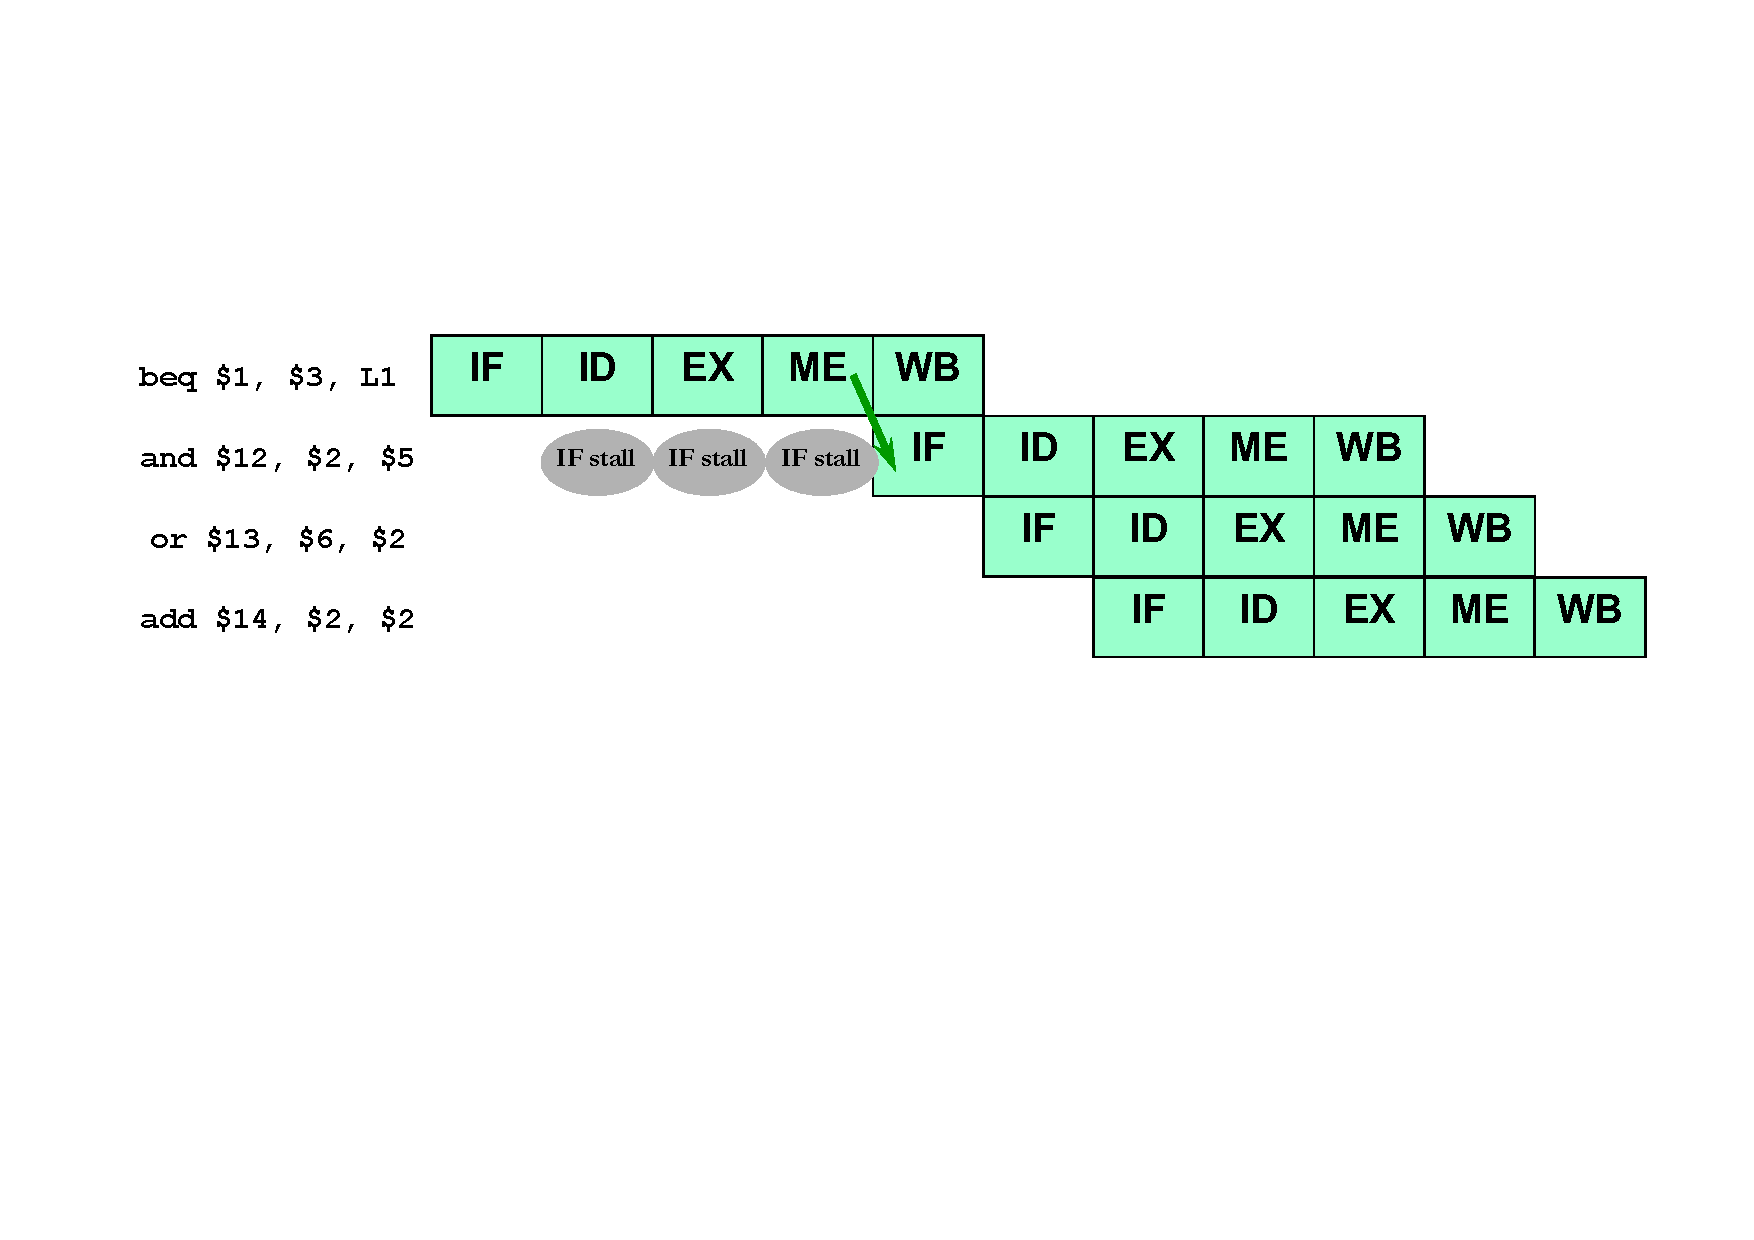
\includegraphics[width=\textwidth]{img/conservative-solution-control-hazards.pdf}
    \caption{\example{Example} of a conservative solution to solve a Control Hazard.}
\end{figure}

\begin{flushleft}
    \textcolor{Green3}{\textbf{\faIcon{check} Start to think to the branch prediction - Flush solution}}
\end{flushleft}
The branch stalls are not good because there is a reduction in throughput. So we can make \emph{a kind of prediction} on the branch and \textbf{assume that the branch will not be taken}. So we start fetching and executing the next 3 instructions in the pipeline. Ok, but wait, \textbf{what if the branch is taken?} No problem, we \textbf{\emph{flush}} the \textbf{next 3 instructions} \underline{before} they write their result and then fetch the instruction at the branch target address.
\begin{figure}[!htp]
    \centering
    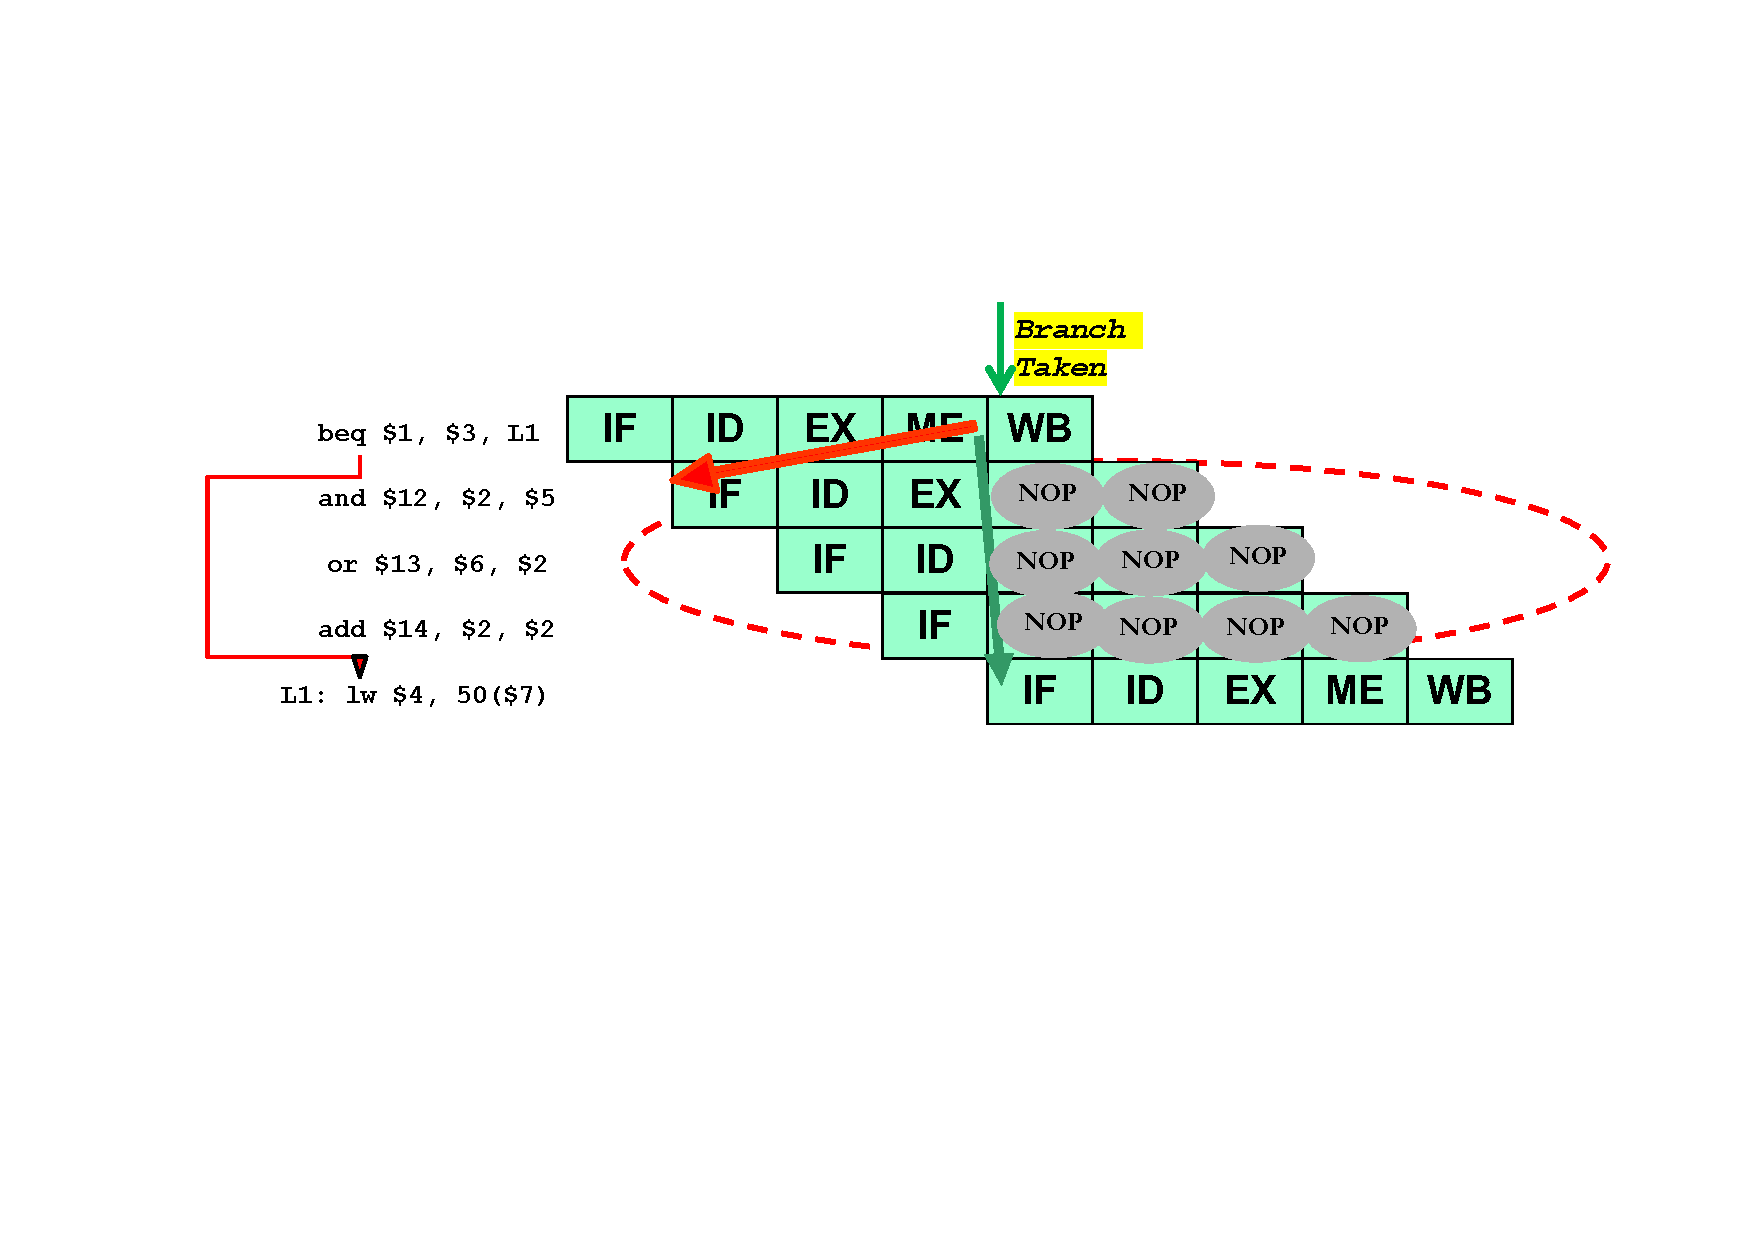
\includegraphics[width=\textwidth]{img/banch-prediciton-control-hazard.pdf}
    \caption{\example{Example} of a flush solution to solve a Control Hazard.}
\end{figure}

\newpage

\begin{flushleft}
    \textcolor{Green3}{\textbf{\faIcon{check} Early Evaluation of the Program Counter (PC) in ID stage}}
\end{flushleft}
It's clear that to improve performance in the event of branch hazards, we need to add more hardware features, such as:
\begin{itemize}
    \item Compare registers to derive the Branch Outcome (BO).
    \item Compute the Branch Target Address (BTA).
    \item Update the PC register.
\end{itemize}
Fortunately, the MIPS-optimized pipeline already has these features and does so during the ID stage. As a result, the \textbf{Branch Outcome} (BO) and the \textbf{Branch Target Address} (BTA) are \textbf{known at the end of the ID stage}.

\begin{figure}[!htp]
    \centering
    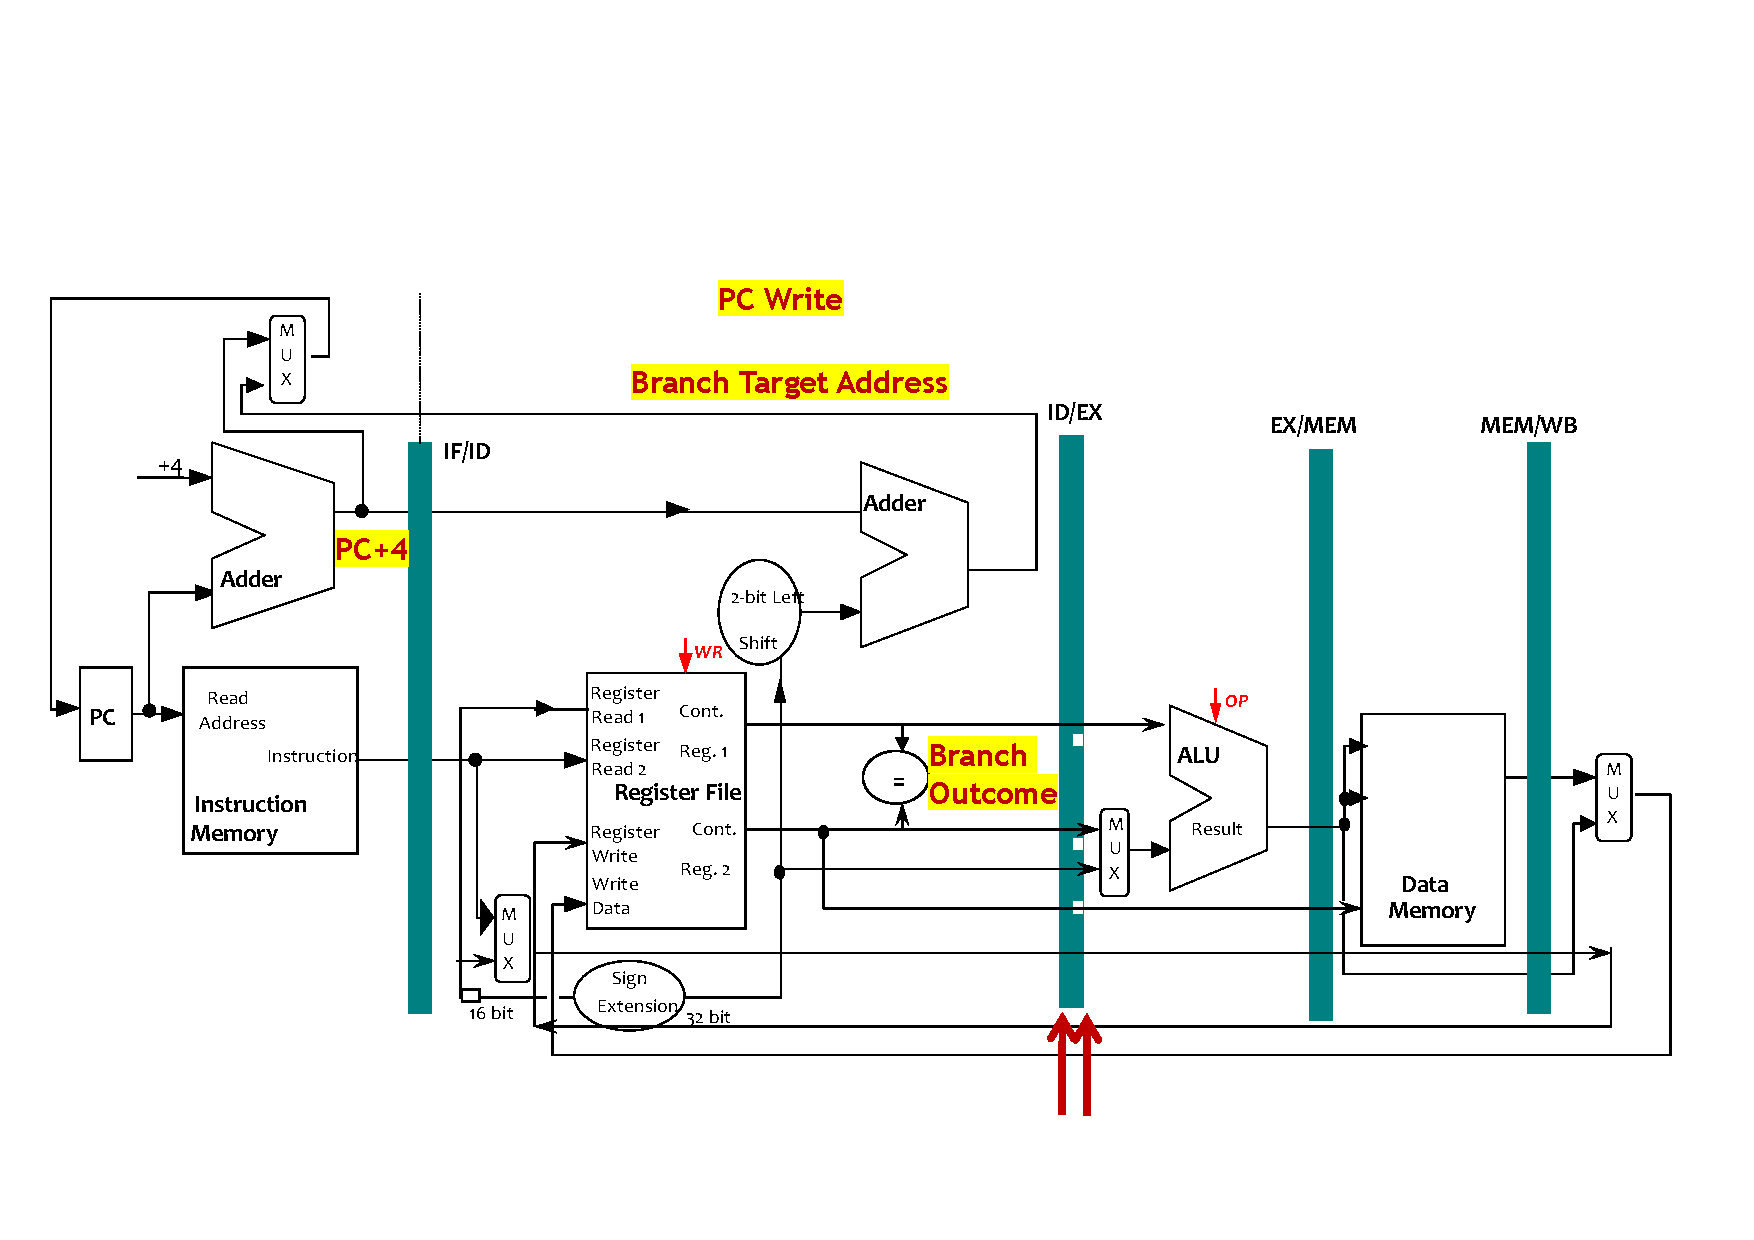
\includegraphics[width=\textwidth]{img/optimization-solution-control-hazard.pdf}
    \caption{Early Evaluation of the Program Counter (PC) in ID stage.}
\end{figure}

\noindent
Now, using the conservative solution or the flush solution, we get two different results:
\begin{itemize}
    \item \textbf{Combo} with \textbf{Conservative Solution}: stalling until resolution at the end of the ID stage (when the Branch Outcome and the Branch Target Address are known) to decide which instruction to fetch.

    \textbf{\emph{Performance consideration}}: each branch costs \textbf{one stall of penalty} to decide and fetch the correct instruction flow along the pipeline.

    One-cycle-delay for every branch still yields a performance loss of 10\% to 30\% depending on the branch frequency (Stall Cycles per Instruction due to Branches equal to Branch Frequency times to Branch Penalty):
    \begin{equation*}
        \texttt{Stall Cycles} = \texttt{Branch Frequency} \times \texttt{Branch Penalty}
    \end{equation*}

    \newpage

    \begin{figure}[!htp]
        \centering
        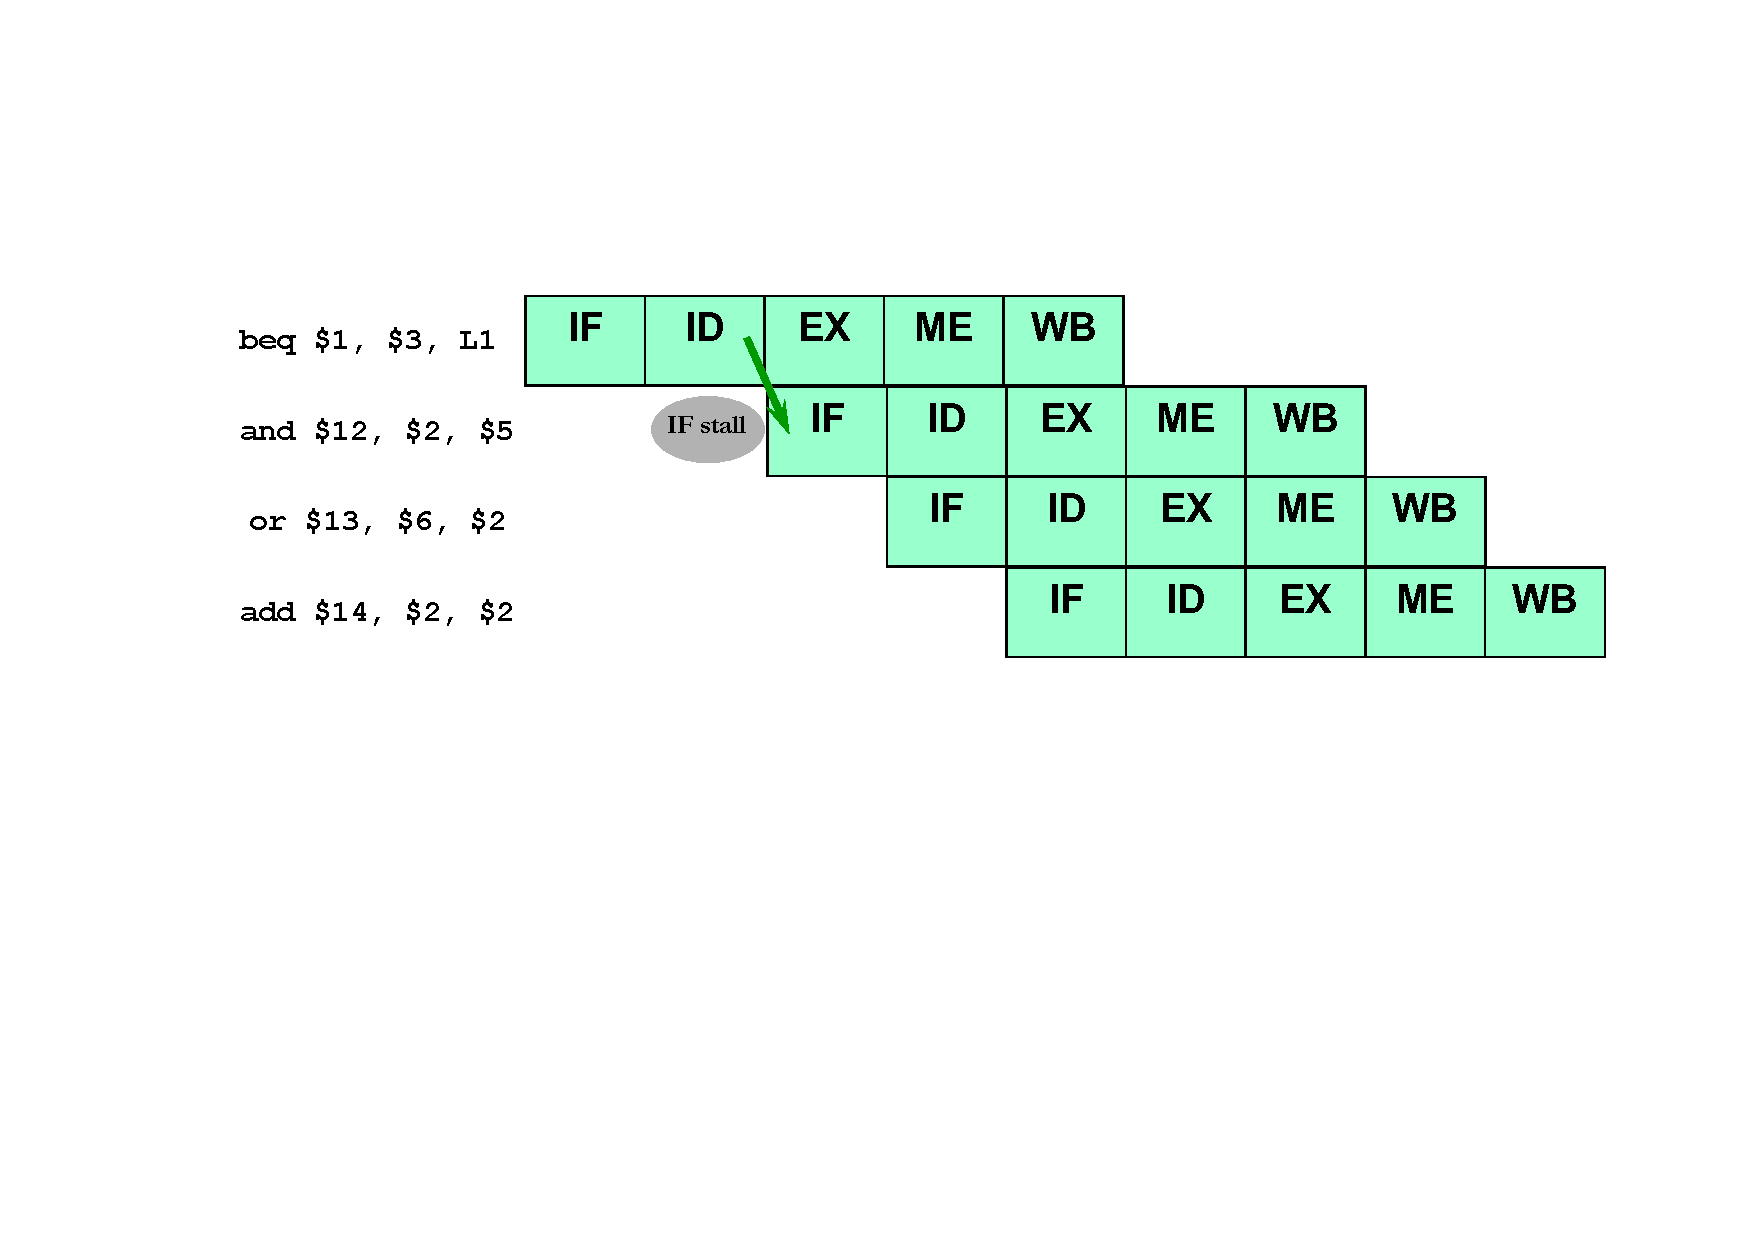
\includegraphics[width=\textwidth]{img/early-evalutation-of-the-pc-1.pdf}
        \caption{\example{Example} of conservative solution in MIPS architecture.}
    \end{figure}

    \item \textbf{Combo} with \textbf{Fetch Solution}: we assume the \textbf{branch is not taken}.
    
    \textbf{\emph{Performance consideration}}: if the Branch Outcome (BO) will be taken, it will be necessary \textbf{to flush only one instructions} before writing its results and fetch the right instruction at the Branch Target Address.
    \begin{figure}[!htp]
        \centering
        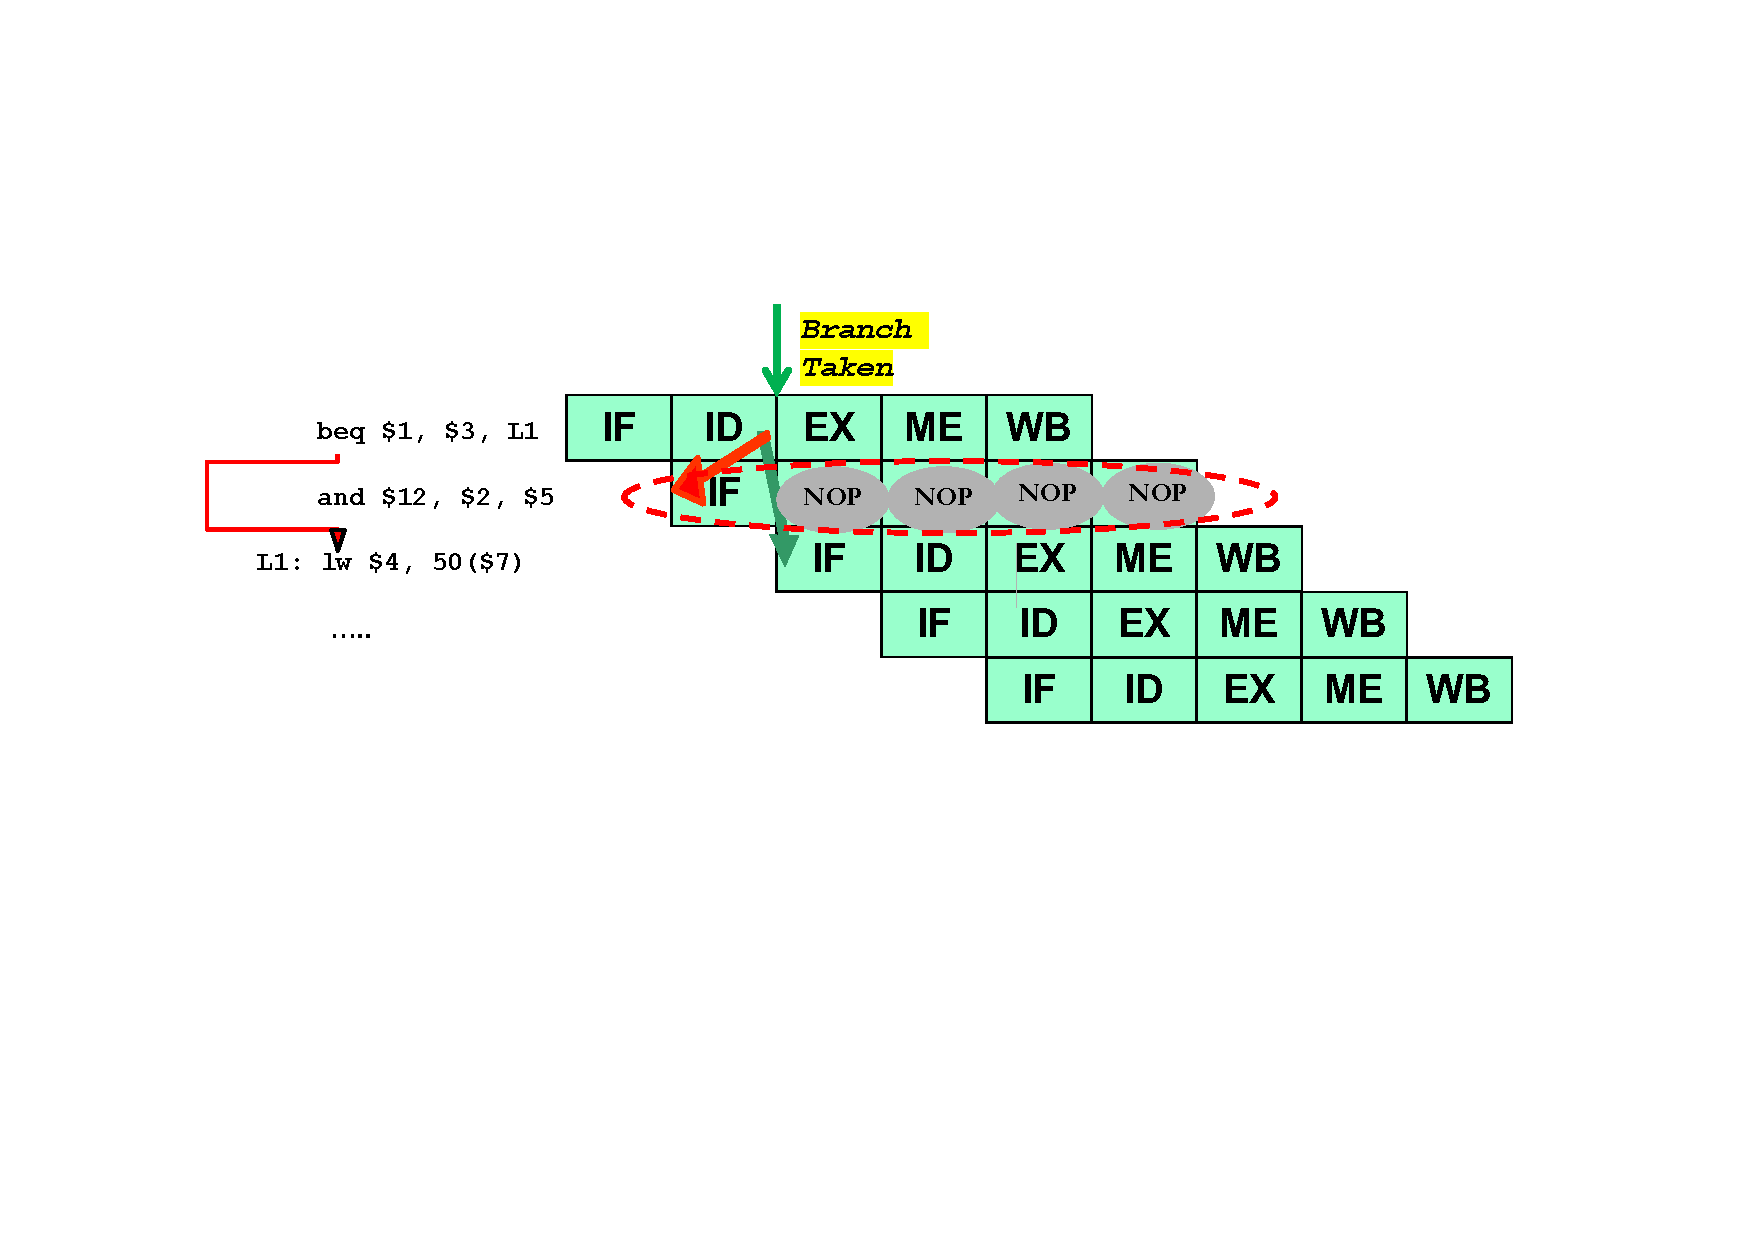
\includegraphics[width=\textwidth]{img/early-evalutation-of-the-pc-2.pdf}
        \caption{\example{Example} of fetch solution in MIPS architecture.}
    \end{figure}
\end{itemize}
The unique solution is to use \textbf{branch prediction techniques} to deal with this loss of performance.